\documentclass[12pt]{article}

\usepackage{amsmath}
\usepackage{amssymb}
\usepackage{amsfonts}
\usepackage[style=iso]{datetime2}
\usepackage[explicit]{titlesec}
\usepackage{amsthm}
\usepackage{array}
\usepackage{graphicx}
\usepackage{float}

\graphicspath{ {./Images/} }

\theoremstyle{definition}
\newtheorem{problem}{Problem}
\newtheorem{definition}{Definition}

\begin{titlepage}
\title{Calculus I: Review of Exponential and Logarithmic Functions}
\author{The Melon Man}
\date{\today}
\end{titlepage}

\renewcommand{\thesection}{\Roman{section}}

\allowdisplaybreaks

\setlength{\parindent}{0pt}
\setlength{\parskip}{1em}

\begin{document}
\maketitle

\section{Exponential Functions}
Exponential functions appear quite often in Calculus.
Let $b$ be a constant and satisfy $b>0$ and $b \neq 1$.
Then, we may define an exponential function $f(x)$ of some variable $x$ as:

\begin{equation}
    f(x) = b^x
\end{equation}

The reason we are avoiding $b=1$ is because that would be a constant function, equivelant to $f(x)=1$.
Having $b=0$ would also lead to a constant function as well.
Having a negative number as the base of an exponential function would require the codomain to be $\mathbb{C}$, the set of complex numbers.
Let's take $b=-2$ as an example.
If $f(x)=(-b)^x$, $f(x)$ would be real for $x$ values such as $x=2$ ($f(x)=4$), it would be complex for $x$ values such as $x=\frac{1}{2}$ ($f(x)=i\sqrt{2}$).
We will avoid this by only allowing $b$ to be greater than 0.

Let's take a look at some exponential functions.

\begin{problem}
Sketch the graph of $f(x)=2^x$ and $\displaystyle g(x)=\left(\frac{1}{2}\right)^x$.
\end{problem}

Let's first create a table of values for the two functions.

\begin{table}[]
    \renewcommand{\arraystretch}{1.5}
    \centering
    \begin{tabular}{>{\centering\arraybackslash}m{1cm}|>{\centering\arraybackslash}m{1cm}|>{\centering\arraybackslash}m{1cm}}
        $x$  & $f(x)$        & $g(x)$        \\ \hline
        $-2$ & $\frac{1}{4}$ & $4$           \\
        $-1$ & $\frac{1}{2}$ & $2$           \\
        $0$  & $1$           & $1$           \\
        $1$  & $2$           & $\frac{1}{2}$ \\
        $2$  & $4$           & $\frac{1}{4}$
    \end{tabular}
\end{table}

Now we may sketch them.

\begin{figure}[H]
    \centering
    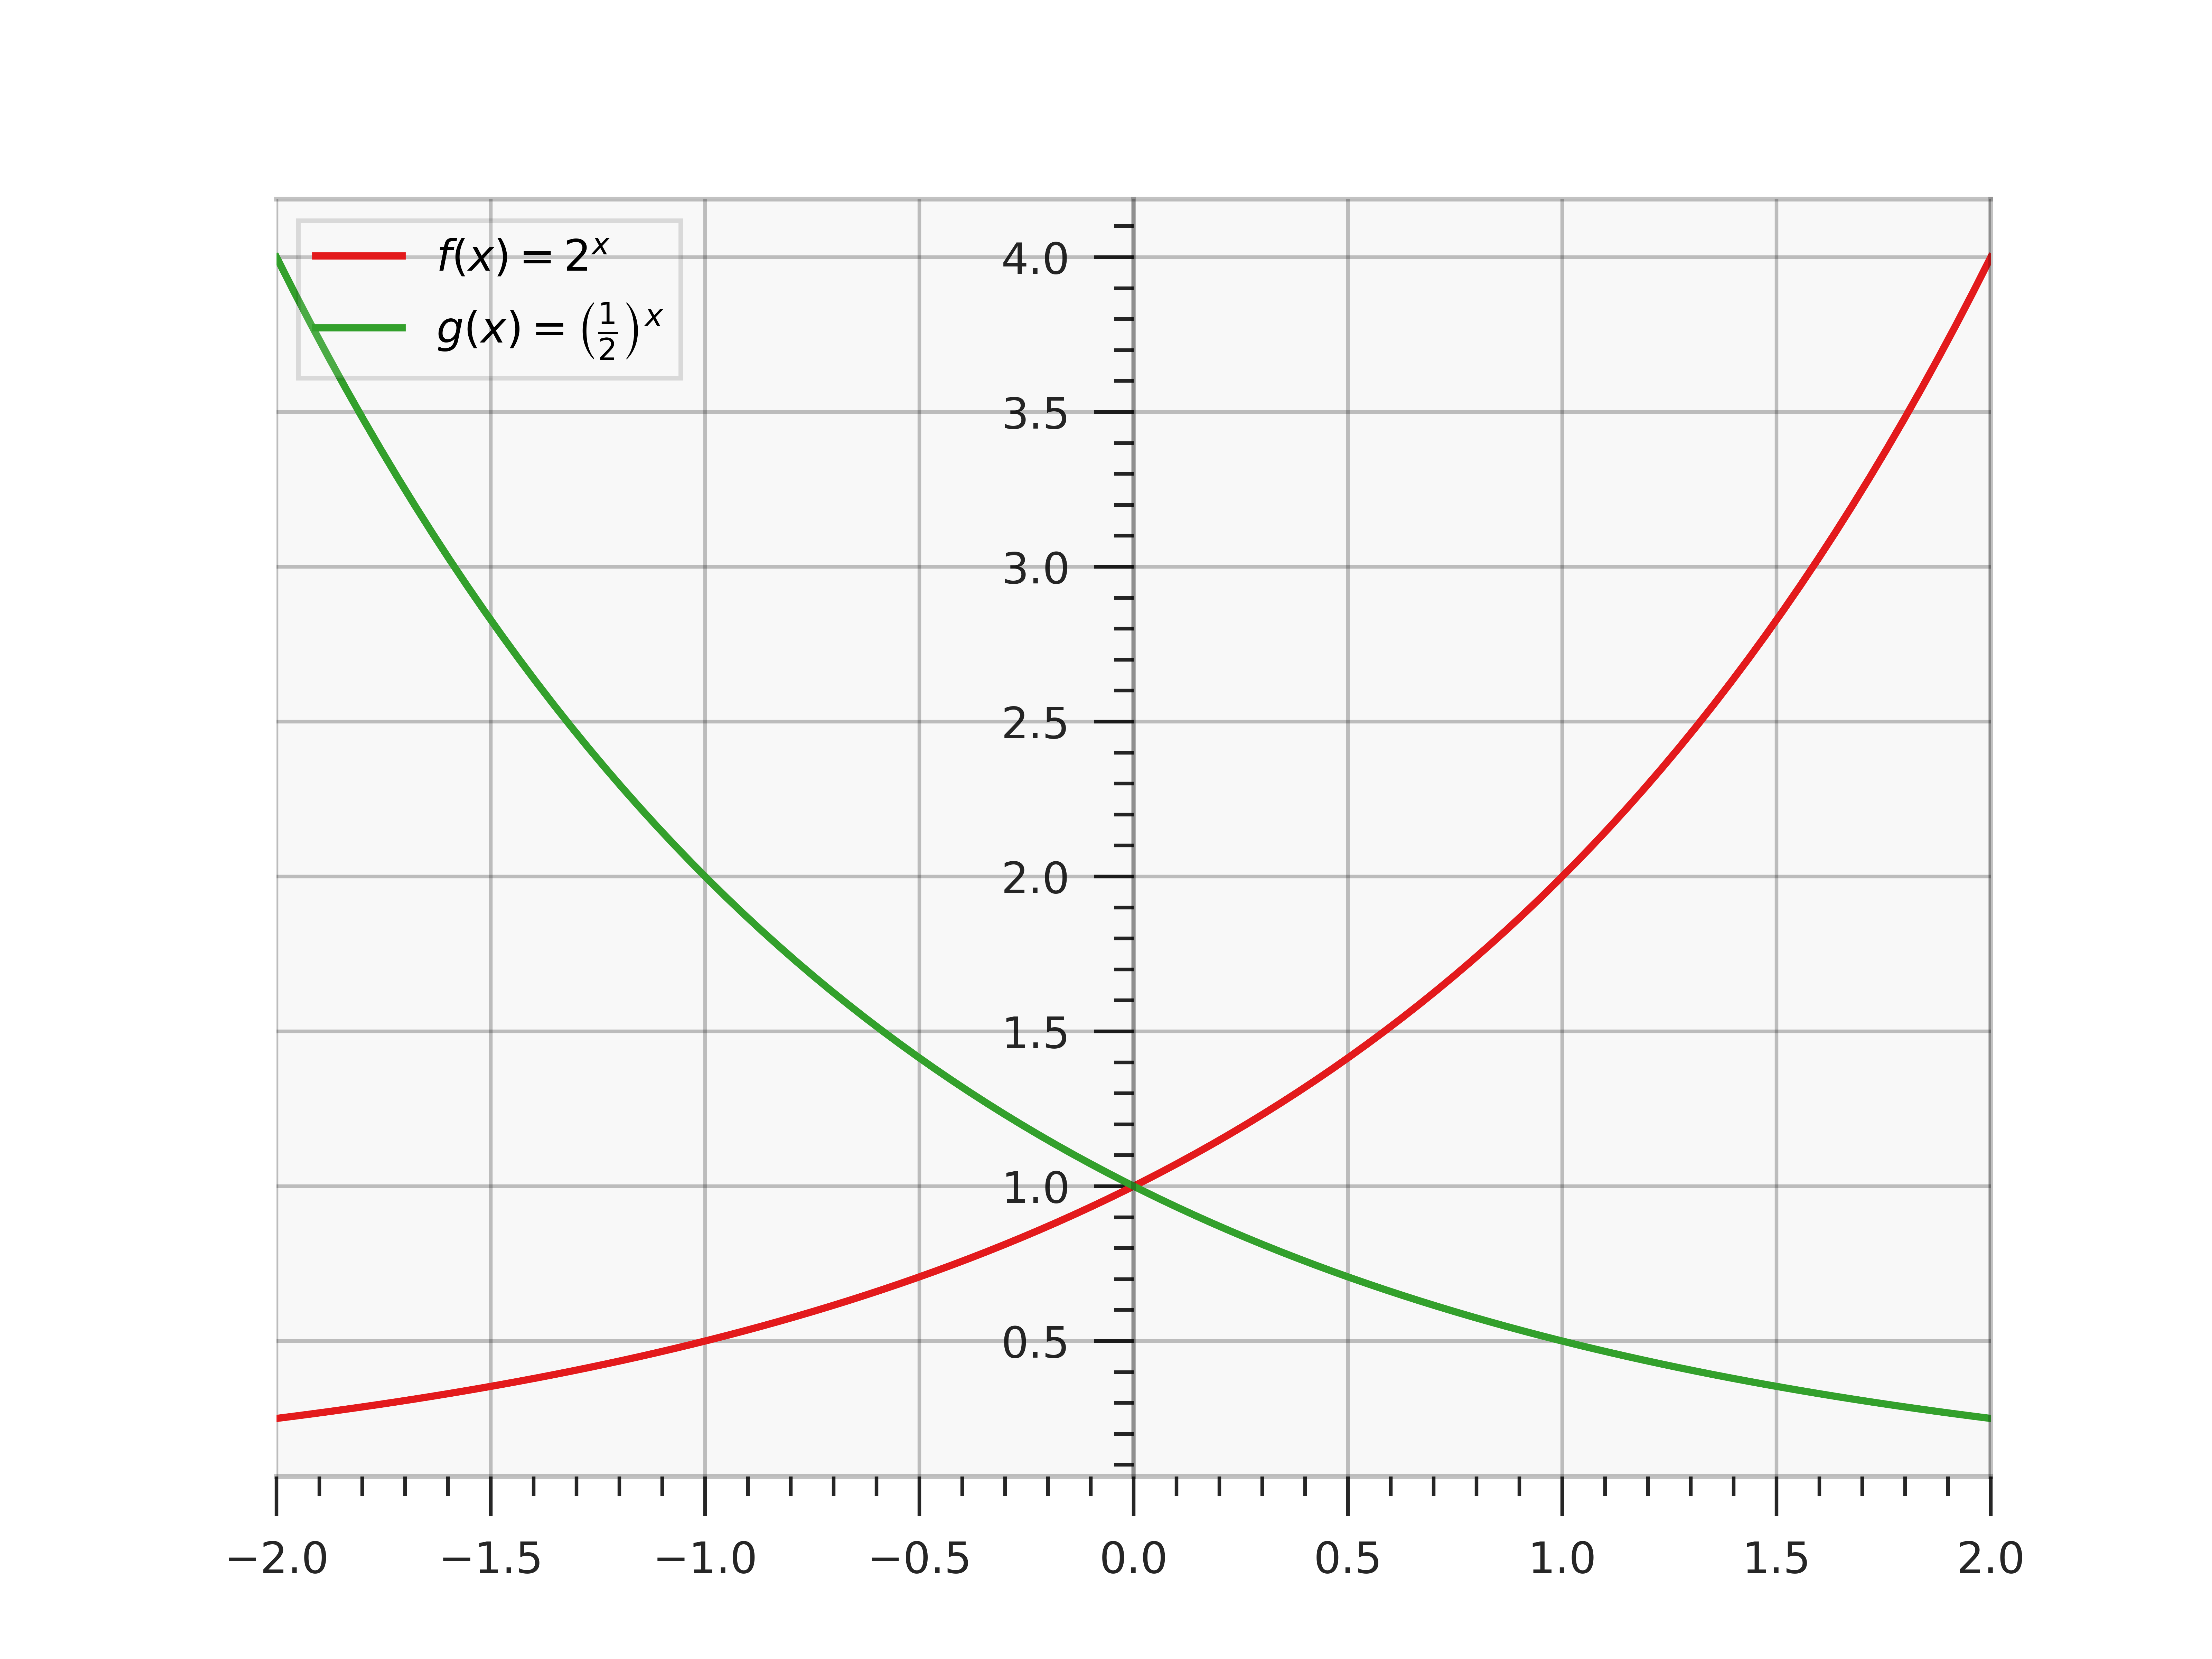
\includegraphics[width=12.5cm, height=10cm]{exponential_functions_1.png}
    \caption{Exponential Functions}
    \label{fig:fig1}
\end{figure}

The graph above highlights some useful properties of exponential functions.
Assuming the equations given above are satisfied, the properties of $f(x)=b^x$ are:

\begin{enumerate}
    \item $f(0) = 1 $. An exponential function will always be 1 at $x=0$.
    \item $f(x) \neq 0$. The function will never be equal to 0.
    \item $f(x) > 0$. The function will always be positive.
    \item The range of an exponential function is $(0, \infty)$.
    \item The domain of an exponential function is $(-\infty, \infty)$.
    \item If $0 < b < 1$, then:
          \begin{enumerate}
              \item $f(x) \rightarrow 0$ as $x \rightarrow \infty$
              \item $f(x) \rightarrow \infty$ as $x \rightarrow -\infty$
          \end{enumerate}
    \item If $b > 1$, then:
          \begin{enumerate}
              \item $f(x) \rightarrow \infty$ as $x \rightarrow \infty$
              \item $f(x) \rightarrow 0$ as $x \rightarrow -\infty$
          \end{enumerate}
\end{enumerate}

These are useful properties to remember throughout a Calculus course.
There is a special type of exponential function, where the base is euler's number, $e$.
This is called the natural exponential function, but is usually just referred to as the exponential function.

\begin{definition}
    The natural exponential function is:
    \begin{equation*}
        f(x) = e^x, e=2.71828182845905 \dots
    \end{equation*}
\end{definition}

As $e>0$, we know that $e^x \rightarrow \infty$ as $x \rightarrow \infty$ and $e^x \rightarrow 0$ as $x \rightarrow -\infty$.
Let's look at an example with this exponential function.

\begin{problem}
Sketch the graph of $h(t) = 1 - 5e^{1-\frac{t}{2}}$.
\end{problem}

Let's make a value table.

\begin{table}[]
    \renewcommand{\arraystretch}{1.5}
    \centering
    \begin{tabular}{>{\centering\arraybackslash}m{1cm}|>{\centering\arraybackslash}m{2cm}}
        $t$  & $h(t)$     \\ \hline
        $-2$ & $-35.9453$ \\
        $-1$ & $-21.4084$ \\
        $0$  & $-12.5914$ \\
        $1$  & $	-7.2436$ \\
        $2$  & $	-4$
    \end{tabular}
\end{table}

We will sketch the above function in our chosen interval.

\begin{figure}[H]
    \centering
    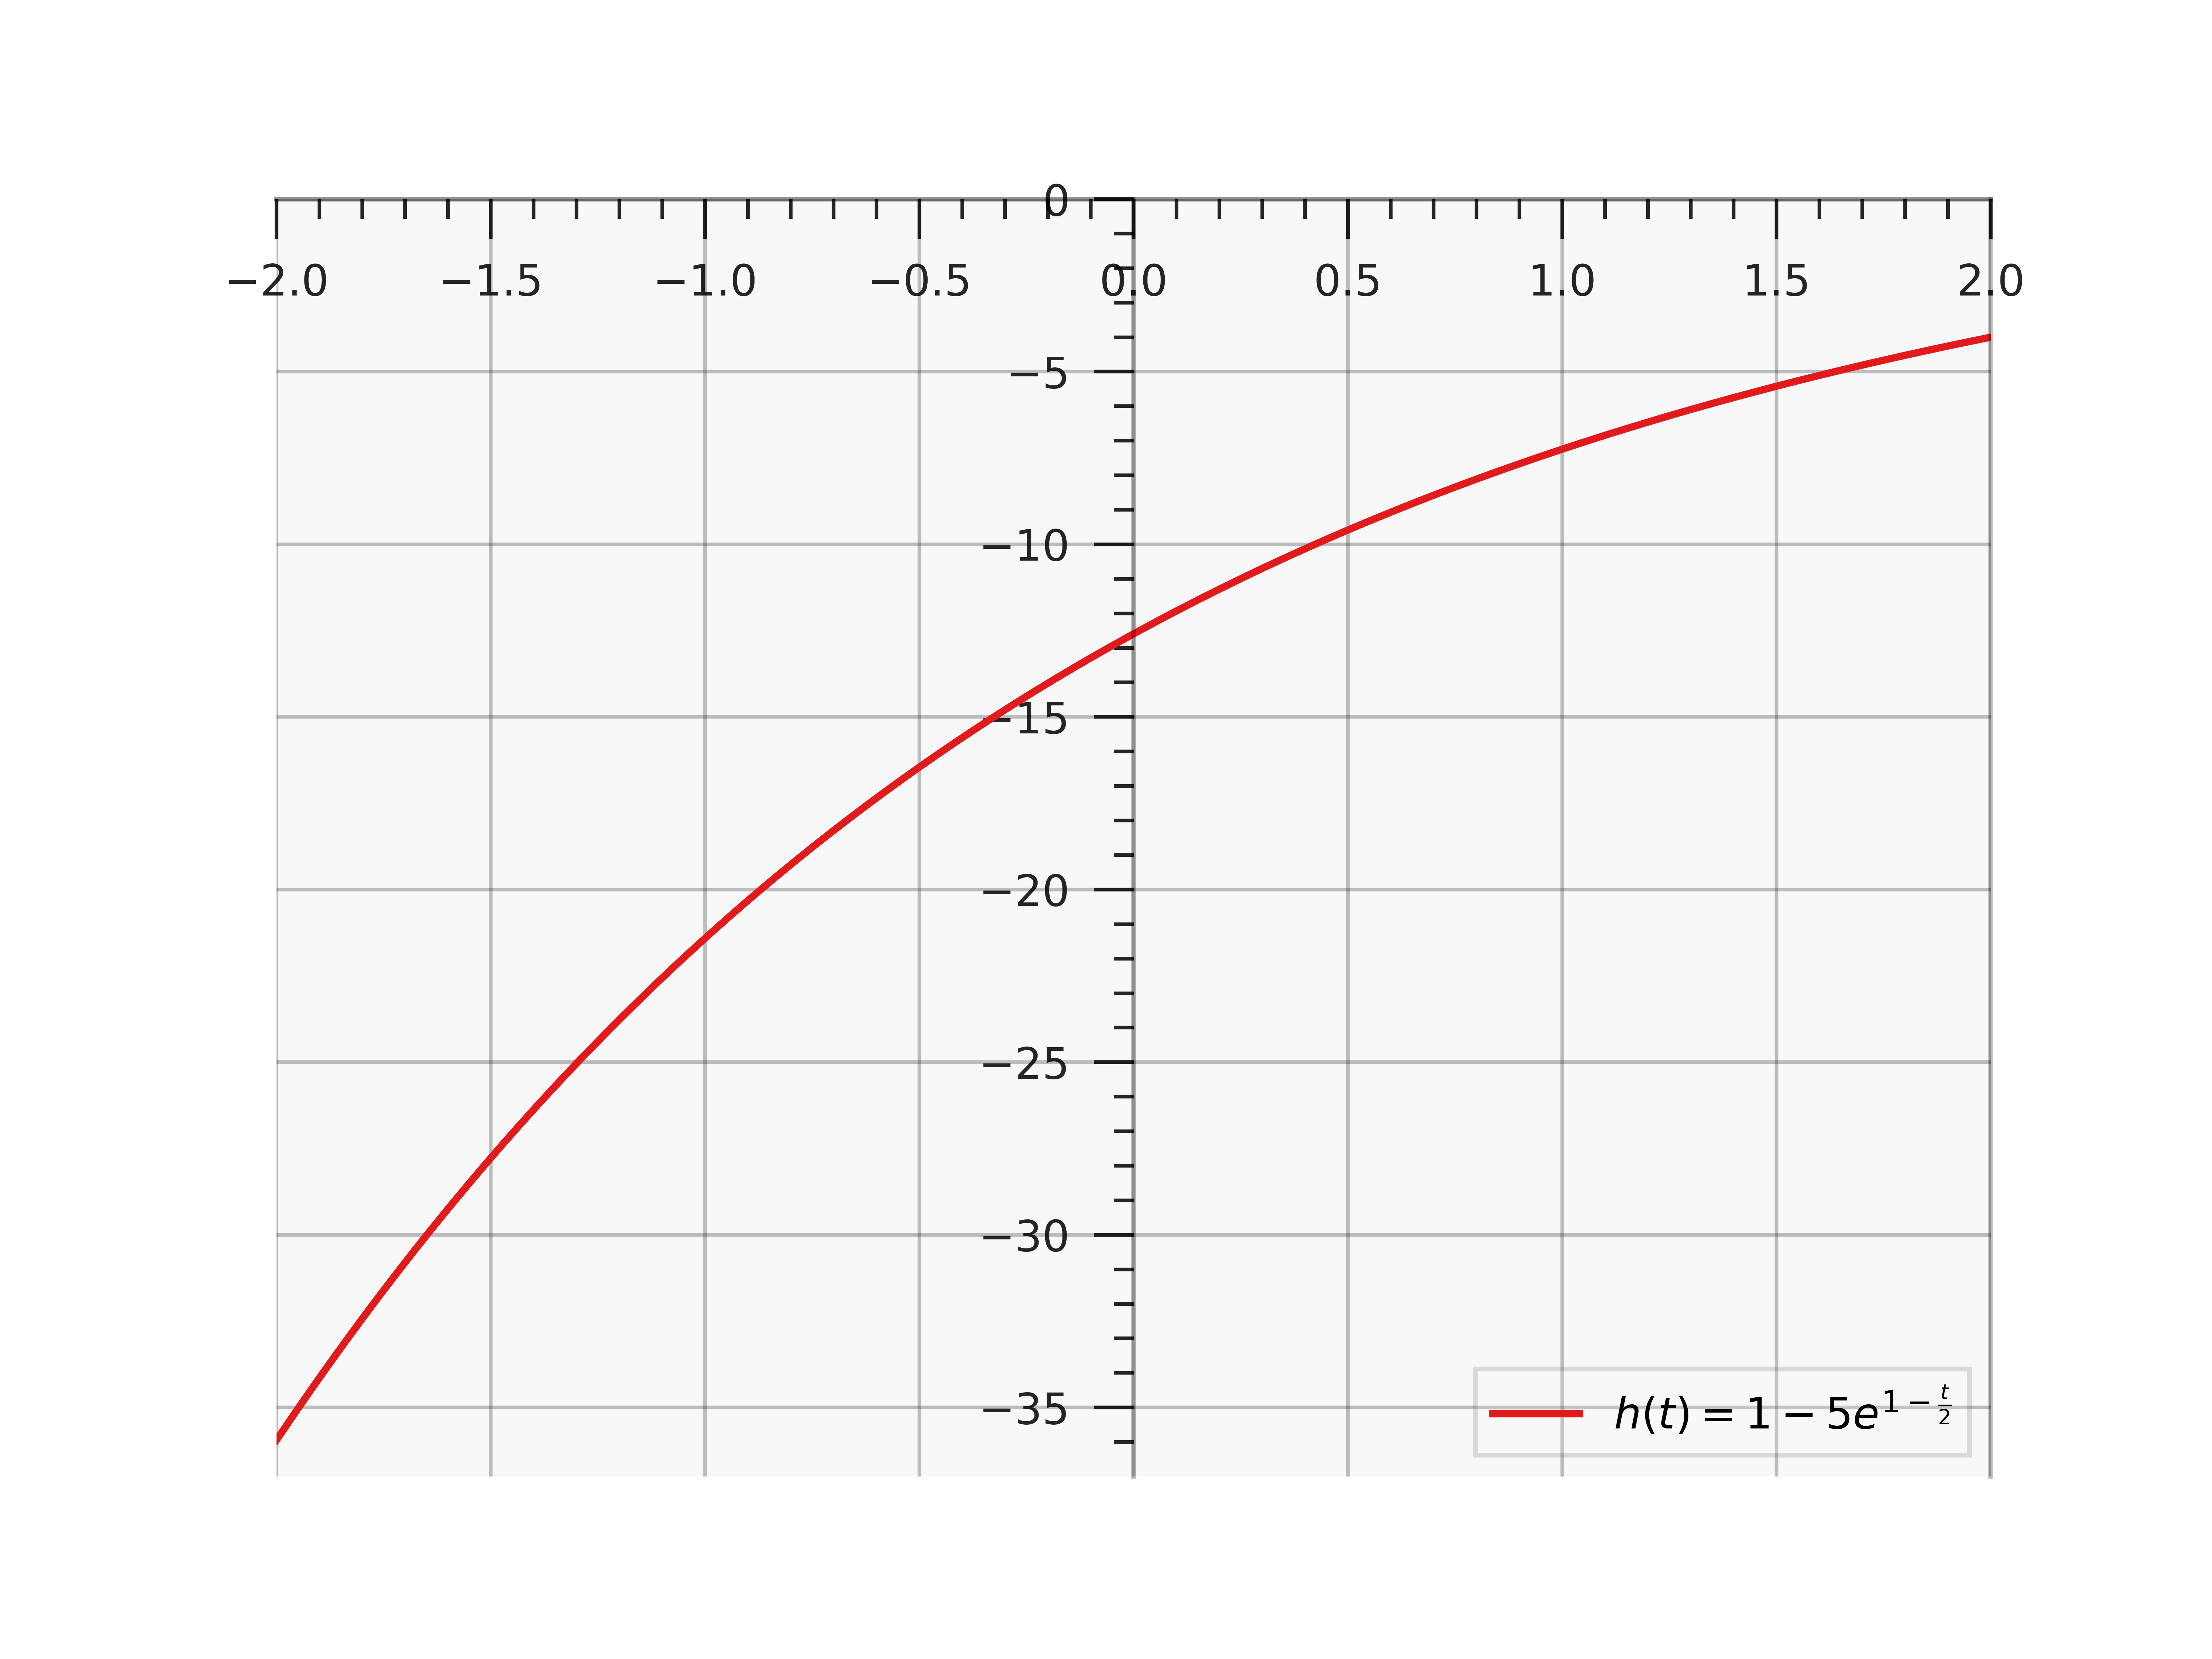
\includegraphics[width=12.5cm, height=10cm]{exponential_functions_2.png}
    \caption{Natural Exponential Functions}
    \label{fig:fig2}
\end{figure}

Being able to evaluate exponential functions is quite important.
Exponential functions will appear in most parts of Calculus I, particularly the natural exponential function.

\section{Logarithmic Functions}

\end{document}